\chapter{Kostenabsch\"atzung f\"ur spritzgussgefertigte Bauteile}
\label{cha:costs}
	
\dictum[David Hilbert]{Im großen Garten der Geometrie kann sich jeder nach seinem Geschmack einen Strauß pflücken.}	
% -------------------------------------------------------------------------------------------------	

\vspace{1cm}
Das Spritzgie{\ss}en (oft umgangssprachlich auch als Spritzguss oder Spritzgussverfahren bezeichnet) ist ein sogenanntes Urformverfahren. Urformen ist ein Oberbegriff f\"ur Fertigungsverfahren, bei denen aus einem formlosen Stoff ein geometrischer bestimmter fester K\"orper hergestellt und der Stoffzusammenhang erzeugt wird. Es werden unter anderem Ausgangstoffe in fl\"ussigem, plastischem oder pulverförmigen Zustand genutzt. Spritzgie{\ss}en wird haupts\"achlich in der Kunststoffverarbeitung, aber auch beim Pulverspritzgie{\ss}en in der Metallverarbeitung eingesetzt.

Mit Hilfe des Verfahrens lassen sich direkt nutzbare Teile in gro{\ss}er St\"uckzahl herstellen. Dazu wir der jeweilige verfl\"ussigte  Werkstoff in eine Werkzeugform unter Druck eingespritzt. Im Werkzeug k\"uhlt der Werksstoff aus und geht wieder in eine feste Form \"uber, so das er nach dem \"Offenen der Form entnommen werden kann. Diese Werkzeugform definiert die Form und die Oberfl\"achenstruktur des zu fertigenden Bauteils. Mit dem Spritzgu{\ss}verfahren lassen sich Bauteile mit sehr geringen Toleranzen, also sehr hoher Fertigungsgenauigkeit, in gro{\ss}en Mengen wirtschaftlich produzieren. 

Spritzgie{\ss}en ist allerdings ein aufwendiger Fertigungsprozess, der nur bei hohen St\"uckzahlen wirtschaftlich ist. Hierbei machen die Kosten der Werkzeugh\"ullen ein gro{\ss}en Teil der Aufw\"ande aus. So ist die Rentabilit\"at von spritzgu{\ss}gefertigen Bauteilen sogar bei einfachen Werkzeugen erst bei einer St\"uckzahl von einigen tausend Teilen erreicht. 
Ma{\ss}geblich f\"ur die Kosten der Werkzeugh\"ullen ist die Komplexit\"at der Bauteilgeometrie. Hierbei sind folgende Eigenschaften besondere Kostentreiber: 

\begin{itemize}
\item Die \textit{Abma{\ss}e des Bauteils}. Die Abma{\ss}e des Bauteils, also die minimale und maximale Dicke, die L\"ange und Breite bestimmen die Gr\"osse des ben\"otigten Werkzeugs und sind damit ausschlaggebend f\"ur die Kosten.

\item Anzahl der \textit{Hinterschnitte} oder \textit{Hinterschneidungen}. Ein Hinterschnitt ist ein Konstruktionselement, das frei am Gussteil hervorsteht und so verhindern kann, dass sich dieses aus seiner Gussform entfernen lässt. Meistens wird dies durch Einlegen von kleinen Teilen, sogenannten Losteilen, erreicht, die den Bereich für den Gu{\ss} versperren. Hinterschneidungen stellen ein technisches Problem da, das die Fertigungskosten von Sppritzgussteilen stark erh\"oht. Ein Beispiel f\"ur Hinterschnitte sind Kunststoffhaken, die verwendet werden um das Werkst\"uck an einem anderen Gegenstück einzurasten. 

\item \textit{Dome}. Ein Dom ist eine zylindrische Struktur, die als Verbindungselemente zu anderen Bauteilen dienen. Sie werden im Abschnitt \ref{sec:dome} n\"aher beschrieben.

\item \textit{Rippen}. Verst\"arkungsrippen sind quarderf\"ormige Strukturen, die die Steifigkeit und Festigkeit von Spritzgu{\ss}teilen erhöhen. Auf sie wird im Abschnitt \ref{rips} n\"aher eingegangen.

\end{itemize}

Die beiden folgenden Abschnitte \ref{sec:dome} und \ref{rips} erl\"autern die f\"ur diese Arbeit relevanten Rippen- und Domstrukturen n\"aher. Hierf\"ur werden die gel\"aufigsten Konstrukten abgebildet und deren Auftreten in den von der VW AG f\"ur dieses Projekt zur Verf\"ugung gestellten Beispieldaten gezeigt. 

\section{Dome}
\label{sec:dome}

Ein Dom ist eine zylindrische Struktur, die als Verbindungselement f\"ur andere Bauteile dient.  Hierbei wird der sogenannte F\"ugepartner auf den Dom aufgesteckt. Ein Dom erh\"oht die geometrische Komplexit\"at einer Werkzeugform im Spritzguss ma{\ss}geblich und ist daher ein relevanter Kostentreiber.


Abbildung \ref{im:domes1} zeigt zwei typische, h\"aufig auftretende Domkonstruktionen. Hierbei ist im Bild auf der linken seiten ein einfacher zylindrischer Dom abgebildet, auf der rechten Seite ein zylindrischer Dom mit St\"utzrippen:

\begin{figure}[ht]
    \centering 
    \subfigure[einfacher Dom]{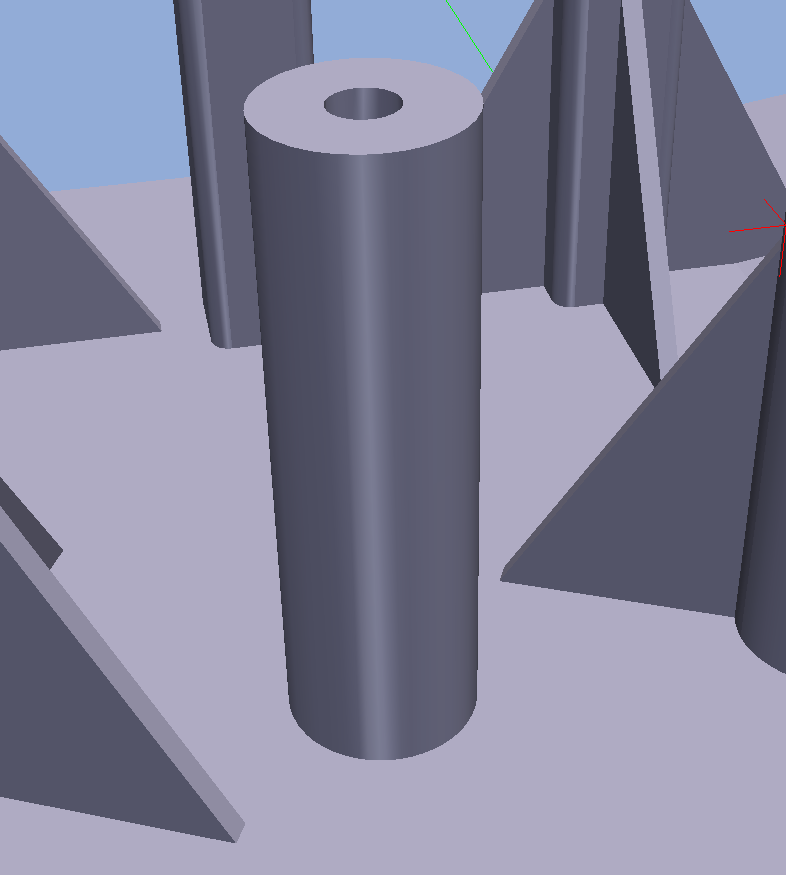
\includegraphics[width=0.3\textwidth]{graphics/simpleDom2.png}} 
    \subfigure[Dom mit St\"utzrippen]{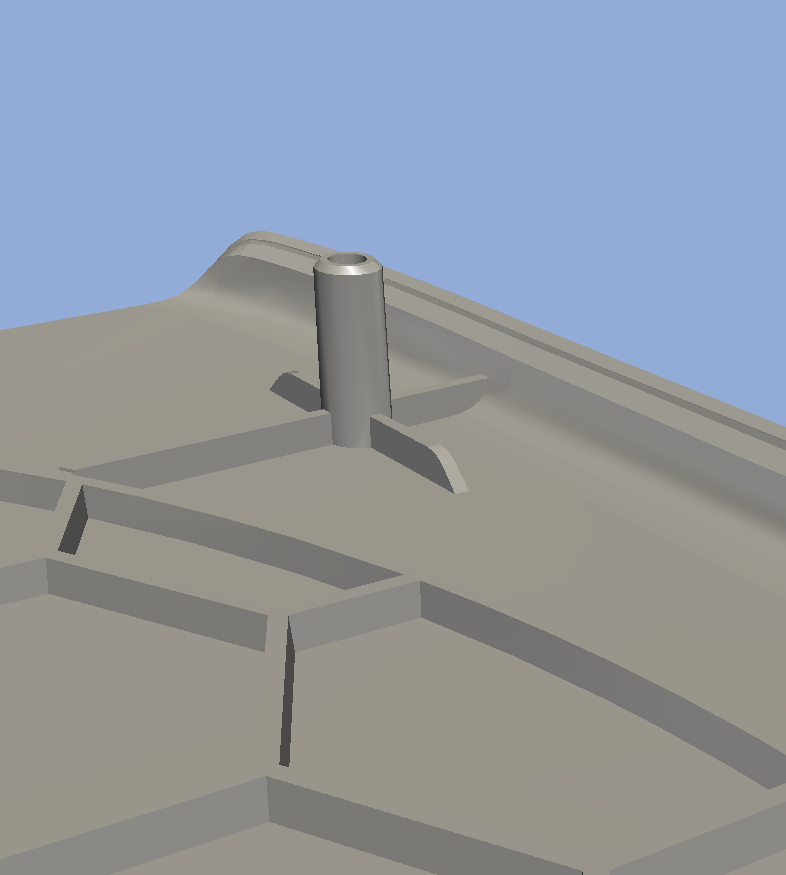
\includegraphics[width=0.3\textwidth]{graphics/ribDom.png}} 
\caption{Einfache Domkonstruktionen.} 
\label{im:domes1}
\end{figure} 


\begin{figure}[ht]
    \centering 
    \subfigure[]{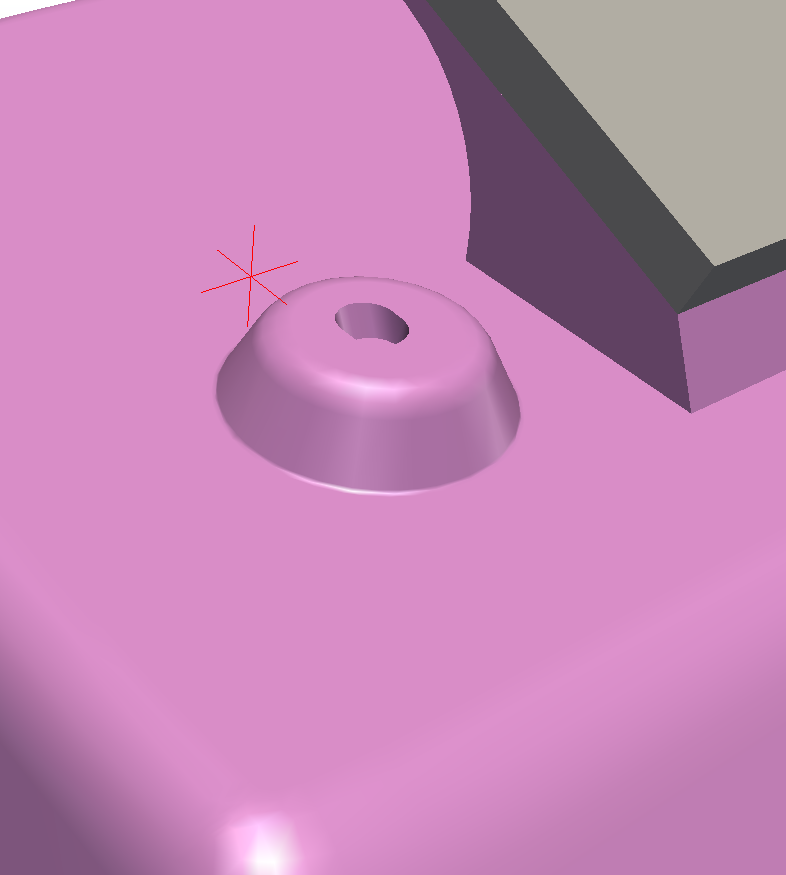
\includegraphics[width=0.23\textwidth]{graphics/domSchraegerMantel.png}} 
    \subfigure[]{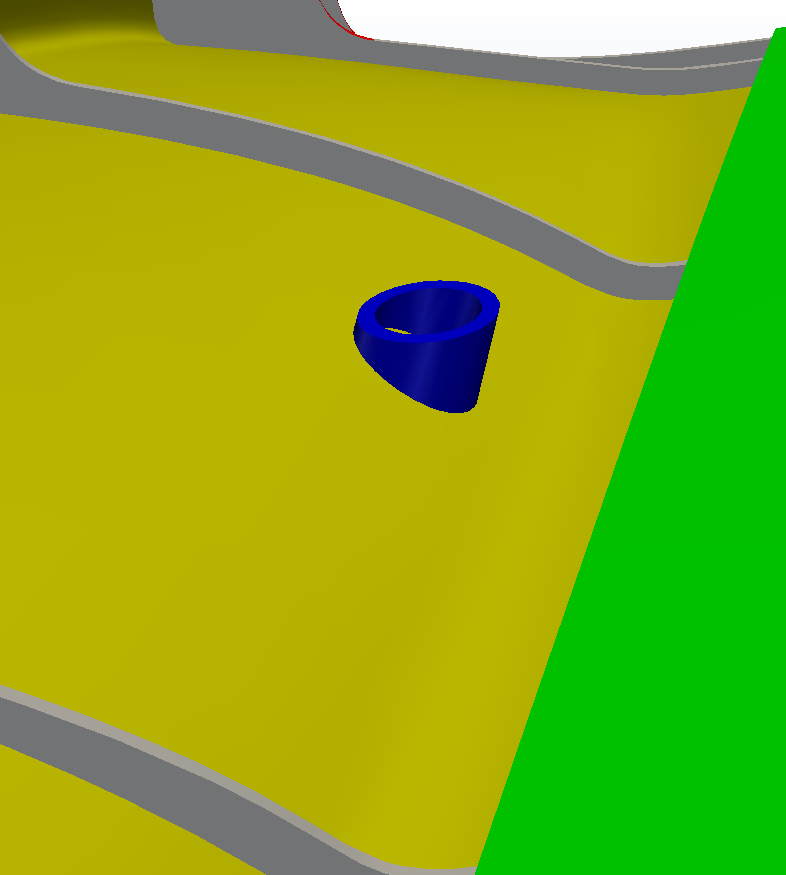
\includegraphics[width=0.23\textwidth]{graphics/domSchraegerBoden.png}} 
    \subfigure[]{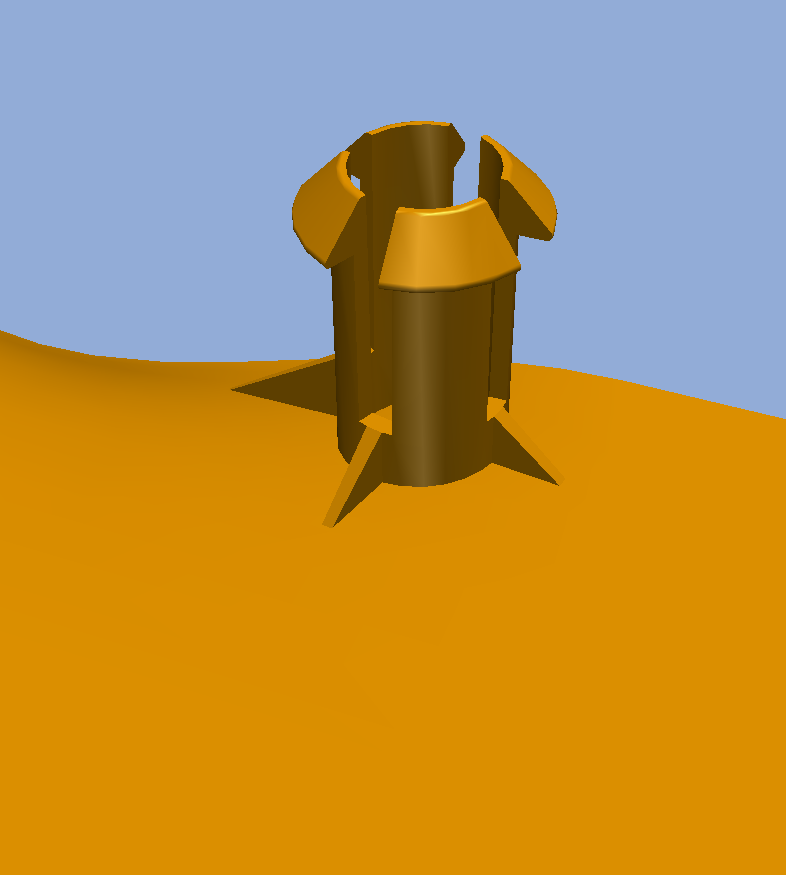
\includegraphics[width=0.23\textwidth]{graphics/complexDom.png}} 
    \subfigure[]{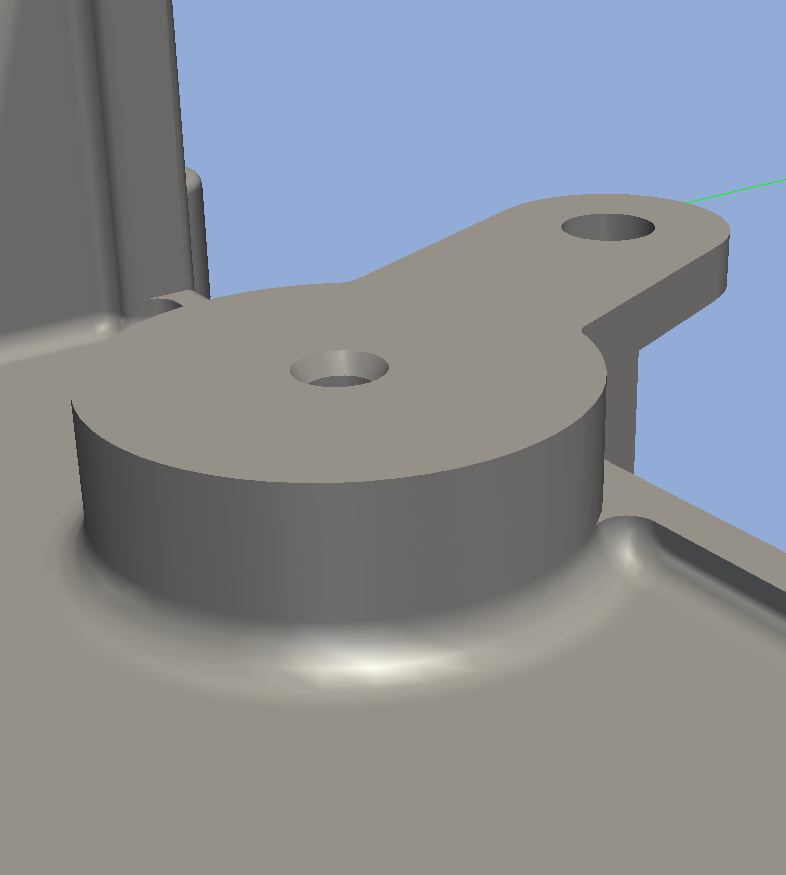
\includegraphics[width=0.23\textwidth]{graphics/domPlane.png}} 
		\subfigure[]{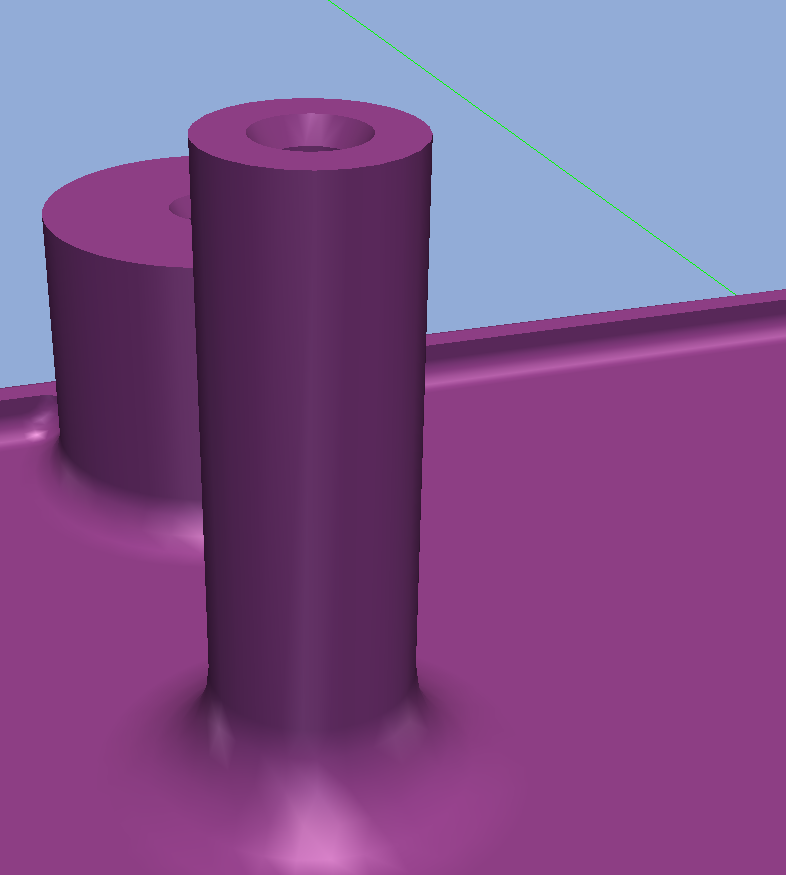
\includegraphics[width=0.23\textwidth]{graphics/domPhaseUnten.png}} 
		\subfigure[]{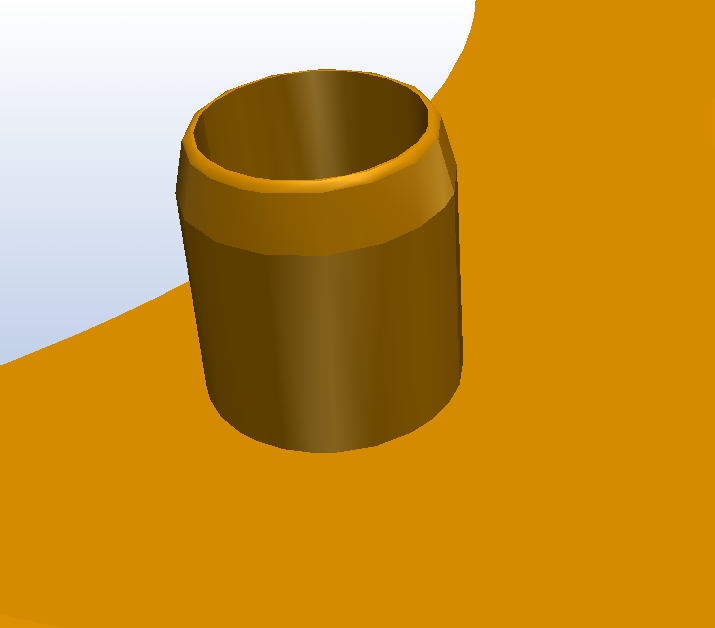
\includegraphics[width=0.23\textwidth]{graphics/simpleDom.png}} 
\caption{Verschiedene Domkonstruktionen.} 
\label{im:domes2}
\end{figure} 

Hier zeigt \textit{(a)} oben links einen einfachen zylindrischen Dom und \textit{(b)} einen zylindrischen Dom mit stabilisierenden St\"utzrippen. In \textit{(c)} und \textit{(d)} werden komplexere Domstrukturen, die aus mehreren geometrischen Grundk\"orpern zusammengesetzt sind, dargestellt. In den Abbildungen \textit{(e)}, \textit{(f)}, \textit{(g)} und \textit{(h)} werden einfache und komplexe Dome in unterschiedlichen geometrischen Kontexten gezeigt: In \textit{(e)} ist ein einfacher zylindrischer Dom auf einer schr\"agen Bodenplatte konstruiert, \textit{(f)} zeigt ein Dom, dessen planare Oberseite direkt in ein planares Element des Bauteils \"ubergeht, die planare Oberseite des Doms in Abbildung \textit{(g)} ist bez\"uglich der Ausrichtung des Doms schr\"ag geneigt. Abbildung \textit{(h)} zeigt einen Dom, der Teilweise mit der Umgebung verbunden ist.  
 
\section{Rippen}
\label{sec:rips}
 
Verst\"arkungsrippen sind ein wirksames Hilfsmittel, um die Steifigkeit und Festigkeit von Spritzgu{\ss}teilen zu erhöhen. Der richtige Einsatz von Rippen kann Material und Gewicht einsparen, die Spritzzyklen verkürzen und dicke Querschnittbereiche vermeiden helfen, die beim Spritzgie{\ss}en zu Problemen führen könnten. Wenn Einfallstellen auf der einer Rippe gegen\"uberliegenden Seite nicht akzeptabel sind, k\"onnen sie durch strukturierte Oberflächen oder andere geeignete Unterbrechungen im Bereich der Einfallstelle kaschiert werden.  

\begin{figure}[H]
\centerline{
	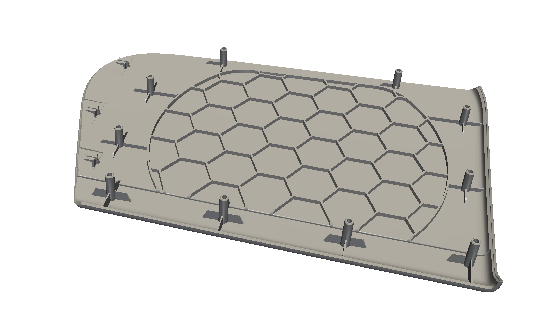
\includegraphics[width=0.8\columnwidth]{graphics/domTeil1.png}}
\caption{Bauteil mit Rippen.}
\label{im:goCart}
\end{figure}

\begin{figure}[ht]
    \centering 
    \subfigure[einfacher Dom]{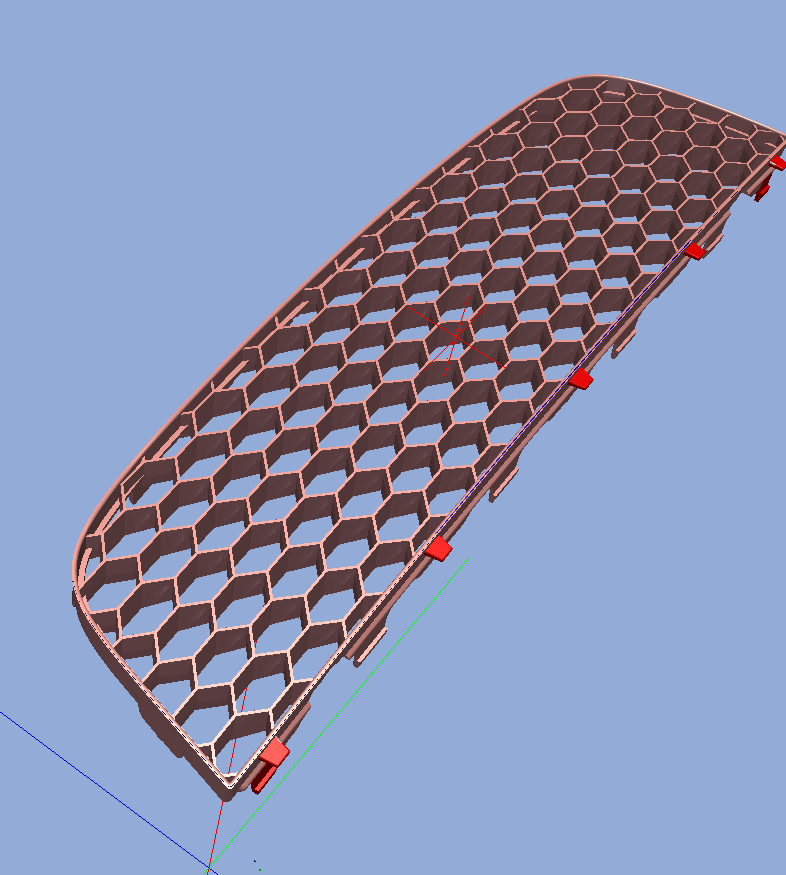
\includegraphics[width=0.24\textwidth]{graphics/ribOffenerBoden.png}} 
		\subfigure[einfacher Dom]{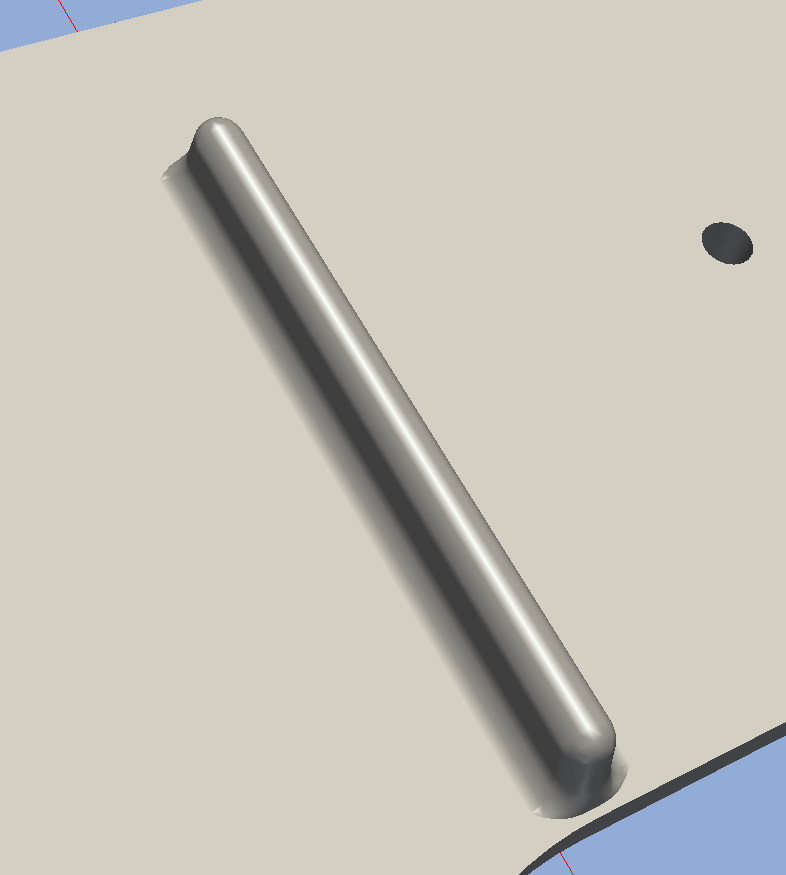
\includegraphics[width=0.24\textwidth]{graphics/angephasteRippe.png}} 
		\subfigure[einfacher Dom]{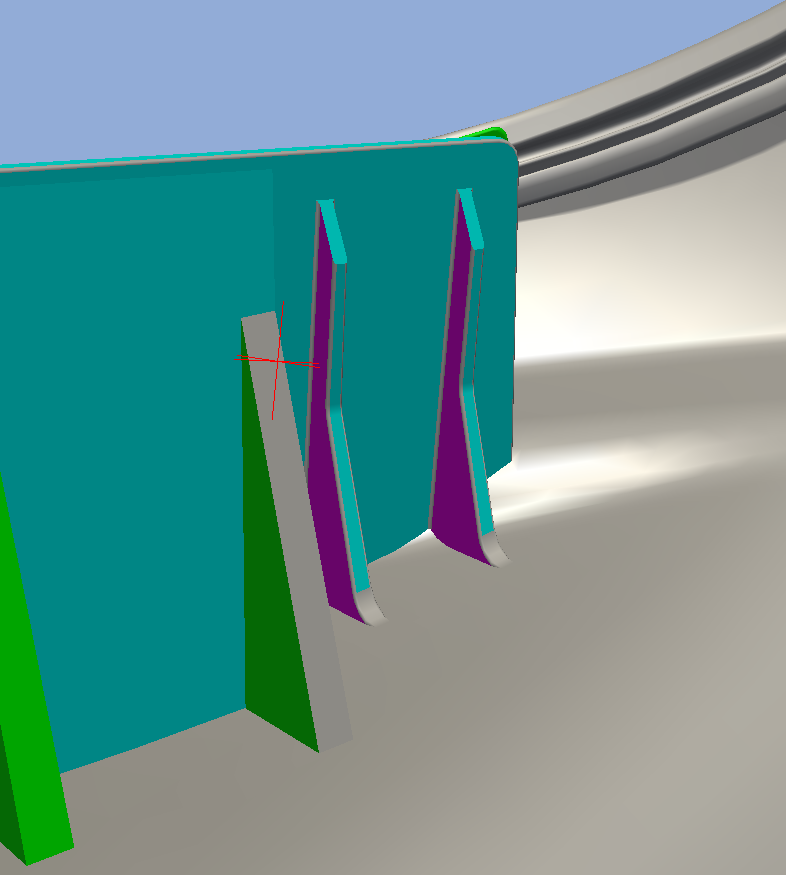
\includegraphics[width=0.24\textwidth]{graphics/komplexeRippe.png}} 
\caption{H\"andisches Ausmessen einer Rippenstruktur} 
\label{im:domes}
\end{figure} 


\section{Das Projekt \textit{GoCart}}
\label{sec:goCart}

\begin{figure}[H]
\centerline{
	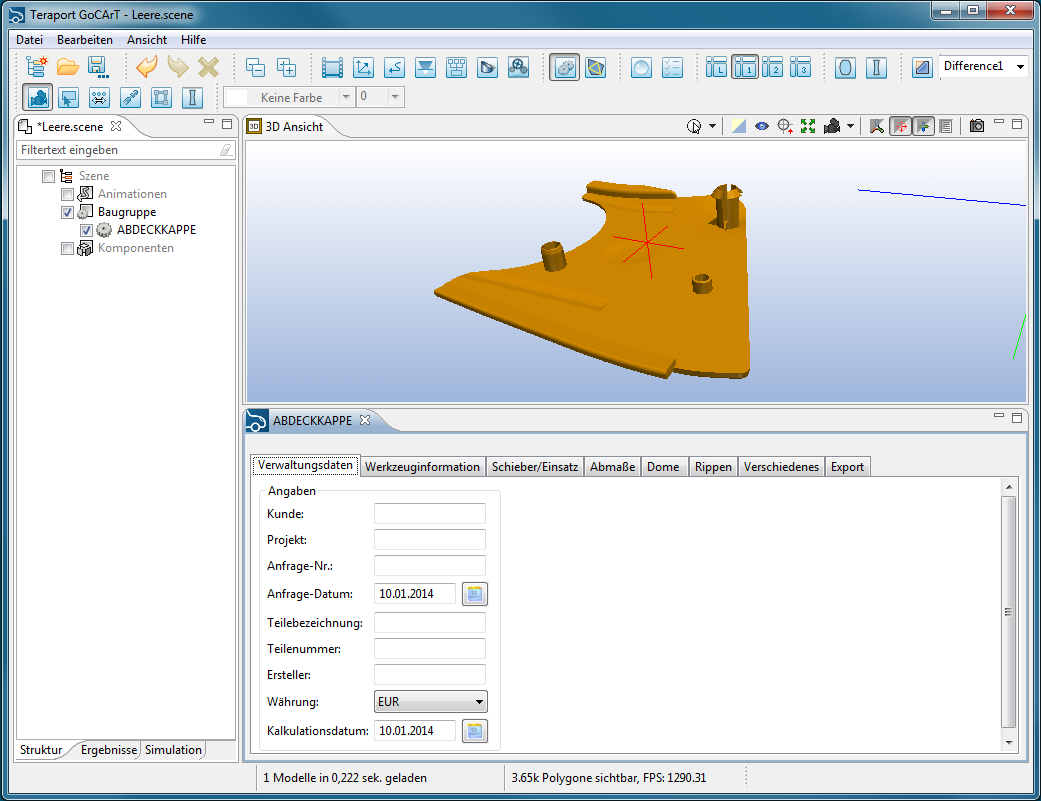
\includegraphics[width=0.95\columnwidth]{graphics/goCart.png}}
\caption{Oberfl\"ache \textit{GoCart}}
\label{im:goCart}
\end{figure}

Der praktische Teil der Masterarbeit wurde im Auftrag der Firma Teraport GmbH erstellt. Dieses Unternehmen besch\"aftigt sich mit der Entwicklung einer Reihe von modularen Softwarebausteinen (dem \textit{DMU-Toolkit}), mit denen sich computergeometische Untersuchungen an triangulierten Fahrzeugdaten durchf\"uhren lassen. Dies sind zum Beispiel die Berechnung von Montagepfaden oder die \"Uberpr\"ufung von umfangreichen Geometrien auf Kollisionen. 

Die Werkzeuge der Teraport GmbH beinhalten auch die Visualisierungsanwendung \textit{DMU.View}, in die einzelne Komponenten des \textit{DMU.Toolkits} integriert werden k\"onnen. Die Anwendung ist bez\"uglich des Funktionsumfangs und des Erscheinungsbild, also beispielsweise des Anwendungsnamens, anpassbar, so das sie gut als Plattform f\"ur individuelle Kundenprojekte eingesetzt werden kann. Ein solches Kundeprojekt ist die Entwicklung der Anwendung \textit{GoCart} f\"ur die VW AG (siehe Abbildung \ref{im:goCart}). Dieses Programm soll das komfortable Erfassen kostenrelevanter Eigenschaften von Spritzgussteilen erm\"oglichen.  

\textit{GoCart} besitzt keine Funktion zur Kalkulation der Kosten eines spritzgu{\ss}gefertigten Bauteils, sondern erfasst ausschlie{\ss}lich hierf\"ur relevante Eigenschaften. Die eigentliche Kalkulation der Bauteilkosten werden mit einer weiteren Anwendung, der \textit{Schmale-Werkzeug kostenkalkulation} der Schmale Werkzeug- und Formtechnik GmbH, durchgef\"uhrt. Mit diesem Programm k\"onnen die relevanten Bauteilinformationen entweder mittels einer grafischen Benutzeroberfl\"ache vom Benutzer h\"andisch eingegeben oder über eine XML-Schnittstelle importiert werden. \textit{GoCart} erzeugt so eine von der \textit{Schmale-Werkzeugkostenkalkulation} lesbare XML-Datei.

Die Anwendung besitzt Funktionalität zum Laden und Visualisieren von triangulierten CAD-Geometrien in üblichen Formaten wie Beispielsweise VRML oder STL, kann aber auch Geometrien, die aus properit\"aren CAD-Systemen wie Catia oder ProE exportiert wurden, lesen. Dar\"uber hinaus wurde Funktionalit\"at zum einfachen Erfassen der von der \textit{Schmale-Werkzeugkostenkalkulation} zur Kostenabsch\"atzung erforderlichen Informationen implementiert. Hiervon sind f\"ur diese Masterarbeit vor allem die Werkzeuge zur Erfassung von Dom- und Rippenstukturen interessant, die in den beiden folgenden Unterkapiteln n\"aher beschrieben werden.


\subsection{H\"andisches Ausmessen von Domstrukturen}
\label{domeMeasure}

\begin{figure}[ht]
    \centering 
    \subfigure[]{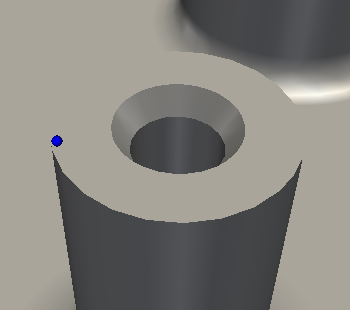
\includegraphics[width=0.22\textwidth]{graphics/dom1.png}} 
		\subfigure[]{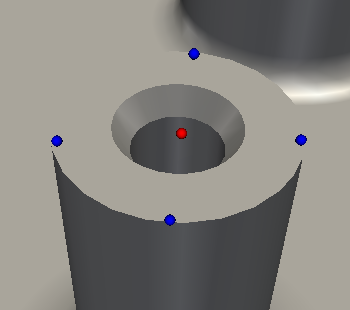
\includegraphics[width=0.22\textwidth]{graphics/dom2.png}} 
		\subfigure[]{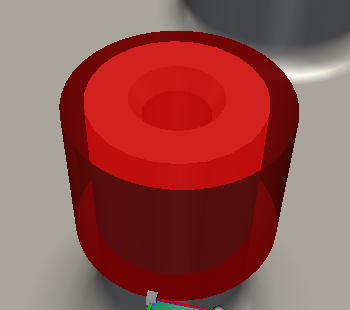
\includegraphics[width=0.22\textwidth]{graphics/dom3.png}} 
		\subfigure[]{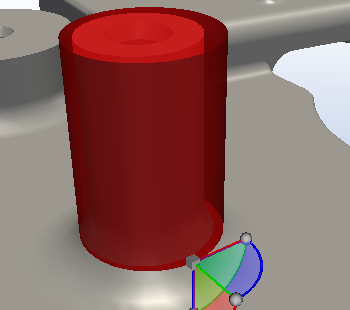
\includegraphics[width=0.22\textwidth]{graphics/dom4.png}} 
\caption{H\"andisches Ausmessen einer Domstruktur.} 
\label{im:domes}
\end{figure} 

Das h\"andische Messverfahren zur Platzierung eines parametrischen Zylinders erfordert zun\"achst die Eingabe einer beliebigen Anzahl von Punkten auf der planaren Oberfl\"ache der Domstruktur. Hierf\"ur wurde grafisches Werkzeug entwickelt, das es dem Benutzer erlaubt, eine Reihe von dreidimensionalen Kugelobjekten durch Linksklick im 3D-Ansichtsfenster zu erzeugen. Die Koordinate der jeweiligen Kugel wird bestimmt, indem der 3D-Selektionsmechanismus (eng. \textit{Picking}) der Anwendung genutzt wurde, um den Schnittpunkt eines Strahls vom Klickpunkt im Ansichtsfenster auf eine Objektgeometrie zu bestimmen.

Diese Kugeln m\"ussen vom Benutzer kreisf\"ormig auf der Zylinderkappe angeordnet werden. Durch Rechtsklick kann dann ein interaktiver parametrischer Messzylinder, mit dem H\"ohe und Radius manipuliert werden kann, erzeugt werden. Das Zylinderobjekt ist an der Normalen der sogenannten \textit{Best-Fitting Plane} ausgerichtet. Eine \textit{Best-Fitting Plane} f\"ur eine dreidimensionale Punktemenge ist diejenige Ebene, die den aufsummierten orthogonalen Abstand der Punkte zur Ebene minimiert. Sie wird sowohl f\"ur die halbautomatische Erkennung von Domstrukturen als auch f\"ur die Segmentierung der Bauteile, die in Abschnitt \ref{cha:segment} beschrieben wird, verwendet. Im Rahmen der Masterarbeit wurde das bestehende, auf Singulärwertzerlegung basierende Verfahren, durch Hauptkomponentenanalyse ersetzt. Es wird im Abschnitt \ref{subsec:pca} näher beschrieben.

Der Zylinder kann so im Schwerpunkt der Punktwolke und an der Normalen der Best-Fitting Plane ausgerichtet erzeugt werden. Als voreingestellter Radius wird der Abstand des am weitesten zum Schwerpunkt entfernten Punktabstand genutzt.
Der Benutzer kann dann mit Hilfe eines Transformationsmanipulators die Höhe und den Radius weiter anpassen.
%Beschreibung Dom
%Bild Dom



%Bild Rippe


%Beschreibung GoCart
%Schmale
%Bild GUI
%Beschreibung Features


\subsection{H\"andisches Ausmessen von Rippenstrukturen}
\label{ribMeasure}

\begin{figure}[ht]
    \centering 
    \subfigure[einfacher Dom]{
\includegraphics[width=0.24\textwidth]{graphics/rippen1.png}} 
		\subfigure[einfacher Dom]{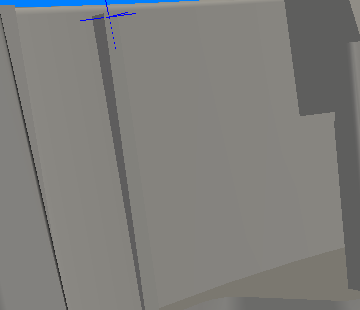
\includegraphics[width=0.24\textwidth]{graphics/rippen2.png}} 
		\subfigure[einfacher Dom]{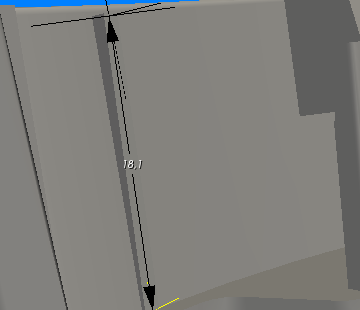
\includegraphics[width=0.24\textwidth]{graphics/rippen3.png}} 
		\subfigure[einfacher Dom]{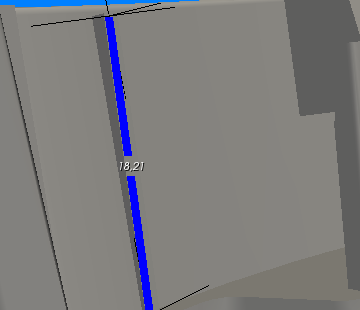
\includegraphics[width=0.24\textwidth]{graphics/rippen4.png}} 
\caption{H\"andisches Ausmessen einer Rippenstruktur} 
\label{im:domes}
\end{figure} 